\begin{figure*}[]
	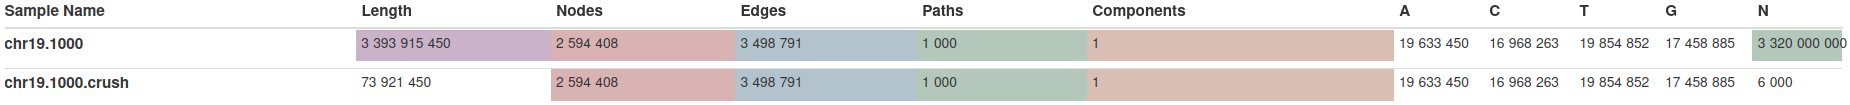
\includegraphics[width=\textwidth]{fig/chr19_multiqc.png}
	\label{fig:chr19_multiqc}
	\caption{Screenshot of the output of ODGI’s MultiQC module displaying the vital graph statistics calculated by odgi stats of the 1000 Genomes Project 1000 haplotypes chromosome 19 pangenome graphs. In the crushed graph consecutive Ns of all nodes containing Ns were merged into just one N per node. A: Number of adenine bases in the graph. C: Number of cytosine bases in the graph. T: Number of thymine bases in the graph. G: Number of guanine bases in the graph. N: Number of bases with unknown base identity.
	}
\end{figure*}